\documentclass[11pt,a4paper]{article}
\usepackage[utf8]{inputenc}
\usepackage[T1]{fontenc}
\usepackage[sc]{mathpazo}
\usepackage[scaled=0.92]{helvet}
\usepackage{microtype}
\usepackage[a4paper,top=2.6cm,bottom=2.4cm,left=2.4cm,right=2.4cm,headheight=14pt]{geometry}
\usepackage[table]{xcolor}
\usepackage{booktabs,array,enumitem,multirow}
\usepackage{tikz}
\usetikzlibrary{calc,positioning}
\usepackage{pgfplots}
\pgfplotsset{compat=1.16}
\usepackage[most]{tcolorbox}
\usepackage{titlesec}
\usepackage{needspace,etoolbox}
\usepackage{fancyhdr}
\usepackage{caption}
\usepackage{url}
\def\UrlBreaks{\do\/\do\-\do\_\do\.\do\=\do\?\do\&\do\a\do\b\do\c\do\d\do\e\do\f\do\g\do\h\do\i\do\j\do\k\do\l\do\m\do\n\do\o\do\p\do\q\do\r\do\s\do\t\do\u\do\v\do\w\do\x\do\y\do\z}
\Urlmuskip=0mu plus 1mu
\urlstyle{same}
\usepackage[hidelinks]{hyperref}

% ---- Palet (selaras dengan halaman dokumen pelengkap) ----
\definecolor{teal}{HTML}{0A6C6E}
\definecolor{tealdark}{HTML}{07484A}
\definecolor{ink}{HTML}{13262A}
\definecolor{muted}{HTML}{51666A}
\definecolor{rule}{HTML}{D3DEDC}
\definecolor{pale}{HTML}{EEF5F4}
\definecolor{amber}{HTML}{B7791F}
\definecolor{amberpale}{HTML}{FBF4E4}
\definecolor{well}{HTML}{CFE3E0}

\renewcommand{\tablename}{Tabel}
\renewcommand{\figurename}{Gambar}
\renewcommand{\refname}{Daftar Pustaka}
\color{ink}
\setlength{\parindent}{0pt}
\setlength{\parskip}{6.5pt plus 1pt}
\linespread{1.06}
\tolerance=1200
\emergencystretch=3em
\hyphenpenalty=1500
\setlist{itemsep=2.5pt,topsep=3pt,parsep=0pt,leftmargin=1.4em}
\setlist[itemize]{label={\color{teal}\textbullet}}
\renewcommand{\arraystretch}{1.22}
\setlength{\tabcolsep}{5pt}
\captionsetup{font={small,sf,color=muted},labelfont={bf,color=teal},labelsep=period,justification=raggedright,singlelinecheck=false,skip=5pt}

% ---- Judul bagian ----
\titleformat{\section}{\sffamily\bfseries\Large\color{ink}}{\color{teal}\thesection}{0.7em}{}[{\color{rule}\titlerule[0.6pt]}]
\titlespacing*{\section}{0pt}{18pt}{9pt}
\titleformat{\subsection}{\sffamily\bfseries\normalsize\color{tealdark}}{\color{teal}\thesubsection}{0.6em}{}
\titlespacing*{\subsection}{0pt}{11pt}{3pt}

% ---- Kepala dan kaki halaman ----
\pagestyle{fancy}
\fancyhf{}
\renewcommand{\headrulewidth}{0pt}
\fancyhead[L]{\sffamily\scriptsize\color{muted}\textsc{Alergen}\ \raisebox{0.15ex}{\tiny$\bullet$}\ Dampak Ekonomi dan Sosial Skala Nasional}
\fancyhead[R]{\sffamily\scriptsize\color{muted}Kit Diagnostik Alergi Berbasis Patch}
\fancyfoot[L]{\sffamily\scriptsize\color{muted}Universitas Airlangga \ $\cdot$ \ IDS000011522}
\fancyfoot[R]{\sffamily\small\bfseries\color{teal}\thepage}
\renewcommand{\headrule}{\color{rule}\hrule width\headwidth height 0.5pt}
\renewcommand{\headrulewidth}{0.5pt}
\fancypagestyle{plain}{\fancyhf{}\renewcommand{\headrulewidth}{0pt}\fancyfoot[R]{\sffamily\small\bfseries\color{teal}\thepage}}

% ---- Tabel ----
\newcommand{\tH}[1]{\textcolor{white}{\sffamily\bfseries\small #1}}
\newcommand{\tabstart}{\small\rowcolors{2}{white}{pale}\arrayrulecolor{rule}}
\newcommand{\hdrrow}{\rowcolor{tealdark}}
\newcolumntype{L}[1]{>{\raggedright\arraybackslash}p{#1}}
\newcolumntype{R}[1]{>{\raggedleft\arraybackslash}p{#1}}
\setlength{\aboverulesep}{0pt}\setlength{\belowrulesep}{0pt}
\renewcommand{\toprule}{\arrayrulecolor{tealdark}\specialrule{0.9pt}{0pt}{0pt}\arrayrulecolor{rule}}
\renewcommand{\bottomrule}{\arrayrulecolor{tealdark}\specialrule{0.9pt}{0pt}{0pt}\arrayrulecolor{rule}}

% ---- Kotak catatan dan kartu angka ----
\newtcolorbox{catatan}[1][Catatan]{enhanced,breakable,colback=amberpale,colframe=amberpale,boxrule=0pt,
  borderline west={2.2pt}{0pt}{amber},arc=1.5pt,left=10pt,right=8pt,top=6pt,bottom=6pt,
  before skip=8pt,after skip=10pt,
  title={\sffamily\bfseries\small\color{amber}\MakeUppercase{#1}},coltitle=amber,
  attach boxed title to top left={yshift=-2mm,xshift=0pt},boxed title style={empty,left=0pt,top=0pt,bottom=0pt},
  fonttitle=\sffamily,coltext=ink,before upper={\vspace{2pt}}}
\newtcolorbox{kartu}[2]{enhanced,colback=pale,colframe=pale,boxrule=0pt,arc=3pt,
  left=8pt,right=6pt,top=6pt,bottom=6pt,halign=left,
  borderline west={2.5pt}{0pt}{teal},
  before upper={{\sffamily\bfseries\LARGE\color{teal}#1}\par\vspace{1pt}},
  fontupper=\sffamily\scriptsize\color{muted},height=1.95cm,valign=top}
\newcommand{\kartuRow}[4]{%
 \begin{tcbraster}[raster columns=#1,raster equal height,raster column skip=7pt,raster row skip=7pt]#2#3#4\end{tcbraster}\vspace{9pt}}

% ---- Sampul ----
\newcommand{\patchmotif}[2]{% #1 skala, #2 warna garis
 \begin{scope}[scale=#1]
 \draw[#2,line width=1.2pt,rounded corners=9pt] (0,0) rectangle (15,6);
 \foreach \r in {0,1}{\foreach \c in {0,...,4}{
   \draw[#2,line width=1pt] ({1.9+\c*2.7},{4.1-\r*2.2}) circle (0.9);}}
 \end{scope}}

\newcommand{\makecover}[5]{% kode, judul, subjudul, tagline, ringkasan satu kalimat
\begin{titlepage}
\thispagestyle{empty}
\begin{tikzpicture}[remember picture,overlay]
 \fill[tealdark] (current page.north west) rectangle ($(current page.north east)+(0,-17.2cm)$);
 \fill[teal!85!tealdark] ($(current page.north east)+(0,-17.2cm)$) -- ($(current page.north east)+(-10cm,-17.2cm)$) -- ($(current page.north east)+(0,-10.8cm)$) -- cycle;
 \begin{scope}[shift={($(current page.north east)+(-9.9cm,-6.4cm)$)}]
   \patchmotif{0.5}{white!35}
 \end{scope}
 \node[anchor=north west,text=white!70,font=\sffamily\small\bfseries,align=left] at ($(current page.north west)+(2.4cm,-2.7cm)$) {\textsc{Alergen \ $\cdot$ \ Universitas Airlangga}};
 \node[anchor=north west,text=white,font=\sffamily\bfseries\fontsize{44}{44}\selectfont] at ($(current page.north west)+(2.4cm,-7.4cm)$) {#1};
 \node[anchor=north west,text=white,font=\sffamily\bfseries\fontsize{26}{31}\selectfont,text width=14.2cm,align=left] at ($(current page.north west)+(2.4cm,-10.2cm)$) {#2};
 \node[anchor=north west,text=white!85,font=\sffamily\fontsize{13}{17}\selectfont,text width=14cm,align=left] at ($(current page.north west)+(2.4cm,-14.1cm)$) {\hyphenpenalty=10000\exhyphenpenalty=10000 #3};
 \node[anchor=north west,text=ink,font=\fontsize{12}{17}\selectfont,text width=15.2cm,align=left] at ($(current page.north west)+(2.4cm,-18.8cm)$) {#4};
 \draw[teal,line width=2pt] ($(current page.north west)+(2.4cm,-21.9cm)$) -- ++(2.2cm,0);
 \node[anchor=north west,text=muted,font=\sffamily\small,text width=15cm,align=left] at ($(current page.north west)+(2.4cm,-22.4cm)$) {%
  \textbf{\color{ink}Kit Diagnostik Alergi Berbasis Patch (Alergen)}\\[3pt]
  Universitas Airlangga, Surabaya\\
  Paten Sederhana IDS000011522\\
  Oktober 2026};
 \node[anchor=south east,text=muted,font=\sffamily\scriptsize,align=right] at ($(current page.south east)+(-2.4cm,1.6cm)$) {#5};
\end{tikzpicture}
\end{titlepage}
\newpage}

\definecolor{sr1}{HTML}{8AA6AB}
\definecolor{sr2}{HTML}{3FA7A3}
\definecolor{sr3}{HTML}{0A6C6E}
\definecolor{sr4}{HTML}{B7791F}
\pgfplotsset{natbase/.style={width=0.95\linewidth,height=6.2cm,
  every axis label/.append style={font=\sffamily\scriptsize,color=muted},
  tick label style={font=\sffamily\scriptsize,color=muted},
  legend style={font=\sffamily\scriptsize,draw=rule,fill=white,at={(0.5,-0.2)},anchor=north},
  grid=major,grid style={color=rule,line width=0.4pt},
  axis line style={color=rule},tick style={color=rule},
  scaled ticks=false,/pgf/number format/.cd,1000 sep={.},fixed,precision=0,/tikz/.cd},
  natplot/.style={natbase,xtick={1,2,3,4,5},xticklabels={2028,2029,2030,2031,2032}}}
\hypersetup{pdftitle={Dampak Ekonomi dan Sosial Skala Nasional},pdfauthor={Tim Alergen, Universitas Airlangga}}

\pretocmd{\section}{\Needspace{7\baselineskip}}{}{}
\pretocmd{\subsection}{\Needspace{4\baselineskip}}{}{}


\begin{document}

\makecover{Dampak}{Dampak Ekonomi dan Sosial Skala Nasional}{Dampak yang dapat diharapkan dari kit diagnostik alergi bagi pasien, fasilitas kesehatan, industri, dan sistem kesehatan Indonesia}{Dokumen ini memisahkan tiga hal: apa yang sudah terukur, apa yang dihitung dari asumsi, dan apa yang masih berupa hipotesis. Produk belum divalidasi pada manusia, sehingga seluruh angka dampak adalah ilustrasi aritmetika dan bukan hasil pengukuran.}{Seluruh angka dihitung dengan skrip yang dapat dijalankan ulang}

\section*{Ringkasan}
\addcontentsline{toc}{section}{Ringkasan}

\kartuRow{4}
{\begin{kartu}{273.600}{}pemeriksaan selama 2028 sampai 2032, skenario nasional dasar\end{kartu}}
{\begin{kartu}{47,0}{}pemeriksaan per 100.000 penduduk pada 2032, skenario nasional dasar\end{kartu}}
{\begin{kartu}{29,39}{}miliar rupiah: selisih biaya pasien selama lima tahun, pembanding konservatif (ilustrasi)\end{kartu}
\begin{kartu}{0}{}dampak yang sudah terukur dari kit ini; validasi klinis belum dilakukan\end{kartu}}

Dampak ekonomi dan sosial diuraikan pada tingkat nasional: pasien dan keluarga, fasilitas kesehatan, produsen dan industri dalam negeri, serta sistem pembiayaan kesehatan. Tiga skenario nasional dan satu skenario regional dari studi kelayakan skala nasional dipakai sebagai kerangka jangkauan.

\begin{itemize}
\item \textbf{Masalah.} Beban penyakit alergi besar secara global (363 juta penderita asma pada 2023), dan data Indonesia menunjukkan sensitisasi alergen yang tinggi pada anak sekolah di kawasan yang diteliti. Data prevalensi alergi makanan tingkat nasional belum tersedia.
\item \textbf{Jangkauan.} Pada skenario nasional dasar, kit dipakai di 1.338 fasilitas pada 2032 dan menjangkau 273.600 pemeriksaan dalam lima tahun. Itu setara 47,0 pemeriksaan per 100.000 penduduk, jadi dampaknya pada tingkat populasi tetap kecil dan terbatas pada pasien yang memang diperiksa.
\item \textbf{Ekonomi pasien.} Kit memuat 10 alergen dengan harga neto Rp150.000, atau Rp15.000 per alergen. Pembanding konservatif adalah panel IgE 54 alergen di RS Royal Progress (Rp40.741 per alergen, setara Rp407.407 untuk 10 alergen). Pembanding panel kecil adalah uji tusuk kulit 10 alergen seharga Rp1.000.000 Pada margin fasilitas 100\%, kit lebih murah Rp107.407 sampai Rp700.000 per pemeriksaan, atau Rp29,39 miliar sampai Rp191,52 miliar selama lima tahun pada skenario nasional dasar.
\item \textbf{Ekonomi industri.} Dampak bagi produsen dan substitusi impor dibahas secara kualitatif, karena alat kesehatan masih didominasi produk impor tetapi porsi diagnostik alergi belum diketahui.
\item \textbf{Sosial.} Hipotesisnya adalah akses pemeriksaan di layanan primer, kenyamanan pemeriksaan anak, dan berkurangnya pantangan makanan yang tidak perlu. Semuanya hanya dapat dinilai setelah uji pada manusia.
\item \textbf{Pengukuran.} Tujuh indikator dengan nilai awal dan frekuensi disusun pada Bagian 5, termasuk indikator pemerataan antarwilayah.
\end{itemize}

\section{Dasar masalah nasional}

\subsection{Beban penyakit alergi}

Organisasi Kesehatan Dunia memperkirakan 363 juta orang hidup dengan asma pada 2023 \cite{who}. Asma bukan alergi makanan, tetapi merupakan penyakit alergi yang paling sering diukur, sehingga dipakai di sini sebagai penanda beban penyakit alergi secara umum.

Untuk Indonesia, prevalensi asma terdiagnosis dokter pada Riskesdas 2018 dilaporkan 2,4\% \cite{riskesdas}. Angka itu kami kutip melalui sumber sekunder, dan nilai pada Tabel 6.1.1 laporan Riskesdas 2018 belum kami periksa langsung. Prevalensi alergi protein susu sapi pada anak Indonesia dilaporkan 2 sampai 7,5\% berdasarkan data Ikatan Dokter Anak Indonesia yang dikutip media \cite{antara}. Kami tidak menemukan survei nasional prevalensi alergi makanan, sehingga jumlah penderita alergi makanan di Indonesia tidak dapat dinyatakan dengan angka yang kokoh. Akibatnya, dokumen ini tidak menghitung jumlah penderita yang dapat dijangkau secara nasional, dan memakai jumlah pemeriksaan sebagai ukuran jangkauan.

\subsection{Data sensitisasi dari Indonesia}

Dua studi terbatas memberi gambaran sensitisasi pada anak dan remaja. Soegiarto dkk. di Surabaya melaporkan uji tusuk kulit positif pada 21,9\% siswa sekolah dasar, 28,95\% siswa sekolah menengah, dan 45,3\% mahasiswa, dengan tungau debu rumah sebagai alergen terbanyak pada kelompok menengah dan mahasiswa \cite{soegiarto}. Norb\"ack dkk. melaporkan 28,2\% dari 380 siswa sekolah menengah pertama di Jawa dan Sumatra tersensitisasi tungau debu rumah, dan 28,2\% memiliki rinitis saat ini \cite{norback}. Kedua studi menilai alergen hirup pada sampel sekolah di kawasan tertentu. Keduanya tidak mewakili populasi nasional, dan tidak menilai alergi makanan.

\subsection{Keterbatasan layanan dan konteks pembiayaan}

Menteri Kesehatan menyatakan pada Mei 2024 bahwa Indonesia membutuhkan sekitar 29.000 sampai 30.000 dokter spesialis, sementara produksinya sekitar 2.700 per tahun \cite{kabarbursa}. Angka itu mencakup seluruh spesialisasi, bukan khusus alergi dan imunologi, sehingga hanya menunjukkan konteks keterbatasan tenaga. Jumlah ahli alergi-imunologi dan sebaran fasilitas yang mampu melakukan uji alergi per provinsi belum kami temukan datanya, dan itu akan dikumpulkan (Bagian~\ref{sec:data}).

Sisi pembiayaan: peserta JKN mencapai 282,7 juta jiwa pada akhir 2025, lebih dari 98\% penduduk \cite{jkn}, dan BPJS Kesehatan bekerja sama dengan 26.759 fasilitas \cite{bpjs}. Hampir seluruh pasien berada dalam sistem ini. Apakah pemeriksaan alergi dengan kit ini akan dijamin belum diketahui, dan tidak diasumsikan.

\section{Kerangka dampak}

Tabel~\ref{tab:rantai} menyusun rantai dari masukan sampai dampak. Status bukti dibuat tegas supaya proyeksi tidak terbaca sebagai hasil pengukuran.

\begin{table}[htbp]
\centering
\caption{Rantai dampak dan status buktinya.}
\label{tab:rantai}
\tabstart
\begin{tabular}{@{}L{2.4cm}L{6.4cm}L{6.1cm}@{}}
\toprule
\hdrrow\tH{Tahap} & \tH{Isi} & \tH{Status bukti} \\
\midrule
Masukan & Patch sepuluh alergen, aplikasi pembaca, paten, mitra produksi dan fasilitas kesehatan & Prototipe dan paten tersedia; mitra, izin edar, dan validasi klinis belum \\
Keluaran & Kit diproduksi dan dipakai di fasilitas kesehatan; jumlah pemeriksaan & Skenario studi kelayakan, bukan hasil penjualan \\
Hasil (outcome) & Tarif pemeriksaan lebih rendah bagi pasien; pemeriksaan tersedia di layanan primer di banyak wilayah; rujukan lebih tepat & Hipotesis; harga kit tercatat, tetapi tarif akhir ke pasien ditentukan fasilitas \\
Dampak & Beban biaya keluarga dan sistem kesehatan berkurang; kualitas hidup pasien membaik; kapasitas industri dalam negeri bertambah & Hipotesis jangka panjang; tidak dihitung dalam dokumen ini \\
\bottomrule
\end{tabular}
\end{table}

Tabel~\ref{tab:pihak} memetakan siapa yang mendapat manfaat dan siapa yang menanggung biaya atau risiko. Pemetaan ini penting karena dampak yang baik bagi satu pihak dapat menjadi beban bagi pihak lain.

\begin{table}[htbp]
\centering
\caption{Pemangku kepentingan, manfaat potensial, dan beban atau risiko.}
\label{tab:pihak}
\tabstart
\begin{tabular}{@{}L{3.2cm}L{6.0cm}L{5.7cm}@{}}
\toprule
\hdrrow\tH{Pihak} & \tH{Manfaat potensial} & \tH{Beban atau risiko} \\
\midrule
Pasien dan keluarga & Biaya pemeriksaan lebih rendah; tanpa penusukan; akses di layanan primer & Hasil keliru bila akurasi belum terbukti; pantangan yang tidak perlu \\
Fasilitas kesehatan & Layanan baru dan margin dari tiap pemeriksaan; rujukan lebih terarah & Pelatihan tenaga; tanggung jawab interpretasi \\
Produsen dan mitra & Pendapatan dari kit; pemanfaatan kapasitas dalam negeri & Investasi validasi dan produksi; risiko regulasi \\
Universitas Airlangga & Hilirisasi hasil riset; royalti dan reputasi & Biaya pengembangan; masa paten terbatas \\
Pemerintah dan JKN & Peluang skrining yang lebih murah; substitusi impor & Beban klaim bila dijamin; pengawasan mutu \\
\bottomrule
\end{tabular}
\end{table}

\section{Dampak ekonomi nasional}

\subsection{Gambaran dari luar negeri}

Zuberbier dkk. memperkirakan penyakit alergi yang tidak tertangani memadai di Uni Eropa menimbulkan biaya tidak langsung yang dapat dihindari sekitar \texteuro 55 sampai 151 miliar per tahun. Per pasien, biaya terapi yang tepat sekitar \texteuro 125 per tahun, atau 5,2\% dari biaya tidak langsung sekitar \texteuro 2.405 pada pasien yang tidak tertangani memadai \cite{zuberbier}. Studi ini mencakup penyakit alergi secara umum, dan membandingkan komponen biaya yang berbeda (biaya terapi terhadap biaya tidak langsung). Studi ini tidak menilai alat diagnosis, sehingga tidak dapat dibaca sebagai penghematan yang dihasilkan kit ini.

Gupta dkk. memperkirakan alergi makanan pada anak di Amerika Serikat menimbulkan biaya sekitar USD 24,8 miliar per tahun, atau USD 4.184 per anak, berdasarkan survei 1.643 pengasuh. Dari jumlah itu, biaya medis langsung USD 4,3 miliar (17\%) dan biaya yang ditanggung keluarga USD 20,5 miliar (83\%) \cite{gupta}. Pesan yang relevan adalah bahwa sebagian besar beban jatuh pada keluarga, bukan pada fasilitas kesehatan. Struktur pembiayaan dan harga di Amerika Serikat berbeda dari Indonesia, sehingga persentase itu tidak dapat dipindahkan begitu saja.

\subsection{Harga per alergen dan selisih biaya pasien}

Kit memuat sepuluh alergen: tungau debu, udang, susu sapi, daging, ayam, telur, gandum, kacang tanah, kelapa, dan polen. Tarif tes alergi pada 10 fasilitas di Surabaya yang dihimpun Alodokter berkisar Rp485.000 sampai Rp3.270.000 \cite{alodokter}, tetapi halaman itu tidak menyebut jenis tes maupun jumlah alergennya. Tarif tersebut karena itu tidak dapat dibandingkan langsung dengan kit sepuluh alergen. Perbandingan yang lebih adil menormalkan harga per alergen.

Rentang harga tes alergi di Indonesia mulai Rp60.000 hingga lebih dari Rp3.500.000, menurut jenis tes, jumlah alergen, dan fasilitas \cite{tim}. Tabel~\ref{tab:alg} memuat harga yang jumlah alergennya diketahui, dari dua kelompok sumber. Kelompok pertama adalah paket IgE Atopy 54 alergen di rumah sakit Royal Progress seharga Rp2.200.000, atau Rp40.741 per alergen, yang bila disetarakan secara pro rata untuk 10 alergen menjadi Rp407.407 \cite{royal}. Kelompok kedua adalah harga panel 10 sampai 54 alergen di Tirta Medical Centre, Siloam, dan RS Mitra Keluarga \cite{tim}.

Panel kecil jauh lebih mahal per alergen. Uji tusuk kulit 10 alergen berharga Rp1.000.000 dan 20 alergen Rp1.450.000 pada rumah sakit yang sama, sehingga tiap alergen tambahan hanya menambah Rp45.000 dan sekitar Rp550.000 adalah komponen tetap per pemeriksaan (hitungan dari dua titik harga pada satu rumah sakit). Harga pro rata dari panel 54 alergen karena itu meremehkan harga tes 10 alergen yang sebenarnya. Kami memakai dua pembanding: konservatif (Rp407.407) dan panel kecil (Rp1.000.000, uji tusuk kulit 10 alergen). Harga neto kit Rp150.000 setara 37\% dari harga per alergen Royal Progress dan 15\% dari harga panel kecil. Dengan margin fasilitas 100\%, angkanya 74\% dan 30\%.

\begin{table}[htbp]
\centering
\caption{Harga per alergen dan setara 10 alergen (pro rata).}
\label{tab:alg}
\tabstart
\begin{tabular}{@{}L{4.6cm}rL{2.9cm}L{2.7cm}L{2.9cm}@{}}
\toprule
\hdrrow\tH{Tes atau produk} & \tH{Alergen} & \tH{Harga} & \tH{Per alergen} & \tH{Setara 10 alergen} \\
\midrule
Kit Alergen, harga neto produsen & 10 & Rp150.000 & Rp15.000 & Rp150.000 \\
Kit Alergen, margin faskes 100\% & 10 & Rp300.000 & Rp30.000 & Rp300.000 \\
\midrule
IgE Atopy, RS Royal Progress (termasuk konsultasi) & 54 & Rp2.200.000 & Rp40.741 & Rp407.407 \\
IgE Atopy, Tirta Medical Centre & 54 & Rp2.540.000 & Rp47.037 & Rp470.370 \\
IgE Atopy, Tirta Medical Centre & 20 & Rp2.329.000 & Rp116.450 & Rp1.164.500 \\
Paket Tes Alergi, Siloam, mulai dari & 20 & Rp2.000.000 & Rp100.000 & Rp1.000.000 \\
Uji tusuk kulit, RS Mitra Keluarga & 20 & Rp1.450.000 & Rp72.500 & Rp725.000 \\
Uji tusuk kulit, RS Mitra Keluarga & 10 & Rp1.000.000 & Rp100.000 & Rp1.000.000 \\
\midrule
Uji tusuk kulit, Medicastore 2009 & 33 & Rp350.000 sampai Rp600.000 & Rp10.606 sampai Rp18.182 & Rp106.061 sampai Rp181.818 \\
IgE spesifik satuan, Medicastore 2009 & 1 & Rp200.000 sampai Rp300.000 & Rp200.000 sampai Rp300.000 & Rp2.000.000 sampai Rp3.000.000 \\
\bottomrule
\end{tabular}
\end{table}

Ada enam hal yang menentukan cara membaca angka ini. Pertama, jenis tes dan cakupan alergen tiap fasilitas dapat berbeda, dan harga antarcabang bervariasi. Kedua, paket Royal Progress termasuk konsultasi dokter, yang menaikkan harga pembanding konservatif. Ketiga, uji tusuk kulit, IgE serum, dan patch berbeda mekanisme, sehingga perbandingan harga bukan perbandingan kinerja. Keempat, harga uji tusuk kulit pada artikel tahun 2009 sudah berusia 17 tahun sehingga tidak dipakai sebagai pembanding \cite{medicastore}. Pada harga itu uji tusuk kulit 33 alergen berkisar Rp10.606 sampai Rp18.182 per alergen, di bawah harga kit (Rp15.000, atau Rp30.000 dengan margin), sedangkan pada daftar harga terbaru uji tusuk kulit panel kecil sekitar Rp100.000 per alergen, di atas harga kit. Perbandingan dengan uji tusuk kulit bergantung pada ukuran panel dan tahun harga; keunggulan kit yang pasti adalah tanpa penusukan dan pembacaan melalui aplikasi. Kelima, Pramita mencantumkan 46 jenis makanan pada tes IgG toleransi makanan \cite{pramita2}, yang bukan tes diagnostik alergi IgE, sehingga tidak dipakai. Klinik Utama DR Indrajana menawarkan patch test kimia 30 alergen dan tes darah Euroimmun hingga 54 alergen pada kisaran Rp1.800.000 sampai Rp2.500.000 \cite{tim}; rentang itu mencakup dua jenis tes, sehingga tidak dihitung per alergen. Keenam, cakupan sepuluh alergen jauh lebih sempit daripada panel 54 sampai 96 alergen \cite{royal,pramita}. Pasien dengan dugaan alergi di luar sepuluh alergen itu tetap memerlukan tes lain.

Tabel~\ref{tab:saving} menghitung selisih terhadap dua pembanding setara 10 alergen, yaitu konservatif (Rp407.407) dan panel kecil (Rp1.000.000), bila fasilitas menambahkan margin 0, 50, dan 100\% pada harga kit. Harga kit baru menyamai pembanding itu bila fasilitas menaikkan harga sebesar 172\% (konservatif) atau 567\% (panel kecil). Pembanding konservatif lebih rendah daripada tarif terendah di Surabaya (Rp485.000), sehingga hasilnya konservatif.

\begin{table}[htbp]
\centering
\caption{Selisih biaya pasien terhadap dua pembanding setara 10 alergen (konservatif Rp407.407, panel kecil Rp1.000.000) menurut margin fasilitas; kolom terakhir untuk 5.000 pemeriksaan.}
\label{tab:saving}
\tabstart
\begin{tabular}{@{}lrrrrr@{}}
\toprule
\hdrrow\tH{Pembanding} & \tH{Margin faskes} & \tH{Harga ke pasien} & \tH{Persen pembanding} & \tH{Selisih per tes} & \tH{Selisih 5.000 tes} \\
\midrule
Konservatif & 0\% & Rp150.000 & 37\% & Rp257.407 & Rp1.287 juta \\
Konservatif & 50\% & Rp225.000 & 55\% & Rp182.407 & Rp912 juta \\
Konservatif & 100\% & Rp300.000 & 74\% & Rp107.407 & Rp537 juta \\
\midrule
Panel kecil & 0\% & Rp150.000 & 15\% & Rp850.000 & Rp4.250 juta \\
Panel kecil & 50\% & Rp225.000 & 22\% & Rp775.000 & Rp3.875 juta \\
Panel kecil & 100\% & Rp300.000 & 30\% & Rp700.000 & Rp3.500 juta \\
\bottomrule
\end{tabular}
\end{table}

\subsection{Dari fasilitas ke skala nasional}

Tabel~\ref{tab:impact} menerapkan selisih per pemeriksaan (margin fasilitas 100\%; Rp107.407 pada pembanding konservatif dan Rp700.000 pada pembanding panel kecil) pada seluruh pemeriksaan tiap skenario studi kelayakan, dengan satu kit untuk satu pemeriksaan (asumsi). Kolom terakhir adalah pendapatan kotor fasilitas dari margin 100\% atas kit, yaitu insentif ekonomi bagi fasilitas untuk mengadopsi.

\begin{table}[htbp]
\centering
\caption{Jangkauan dan nilai agregat ilustratif selama 2028 sampai 2032 (margin faskes 100\%, terhadap dua pembanding setara 10 alergen).}
\label{tab:impact}
\tabstart
\begin{tabular}{@{}L{2.7cm}R{2.2cm}R{1.9cm}R{2.2cm}R{2.2cm}R{2.2cm}@{}}
\toprule
\hdrrow\tH{Skenario} & \tH{Pemeriksaan} & \tH{Per 100.000 (2032)} & \tH{Selisih konservatif (Rp miliar)} & \tH{Selisih panel kecil (Rp miliar)} & \tH{Pendapatan kotor faskes (Rp miliar)} \\
\midrule
Regional & 52.000 & 7,0 & 5,59 & 36,40 & 7,80 \\
Nasional terbatas & 113.100 & 18,8 & 12,15 & 79,17 & 16,96 \\
Nasional dasar & 273.600 & 47,0 & 29,39 & 191,52 & 41,04 \\
Nasional luas & 541.300 & 94,0 & 58,14 & 378,91 & 81,19 \\
\bottomrule
\end{tabular}
\end{table}

\begin{figure}[htbp]
\centering
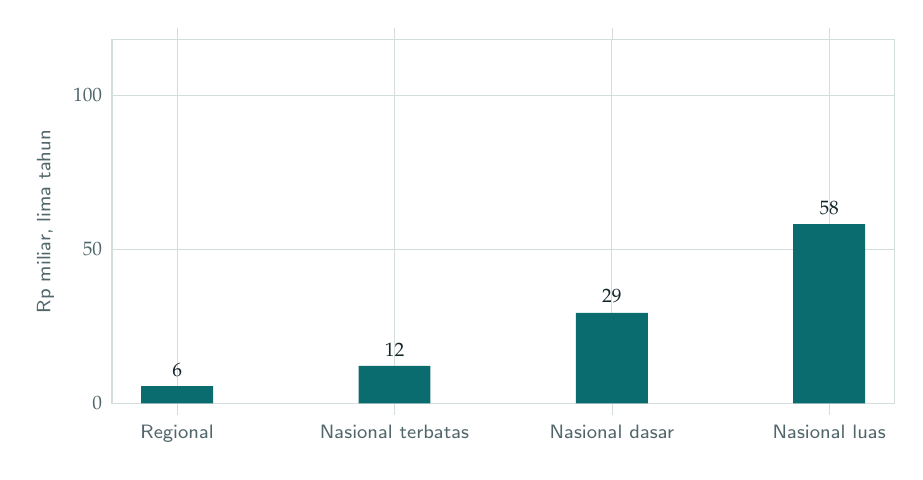
\begin{tikzpicture}
\begin{axis}[natbase,ybar,bar width=26pt,ymin=0,ymax=118,
  symbolic x coords={Regional,Nasional terbatas,Nasional dasar,Nasional luas},xtick=data,
  nodes near coords,every node near coord/.append style={font=\sffamily\scriptsize,color=ink},
  ylabel={Rp miliar, lima tahun},legend style={draw=none,fill=none}]
\addplot[fill=sr3,draw=none] coordinates {(Regional,5.585) (Nasional terbatas,12.148) (Nasional dasar,29.387) (Nasional luas,58.140)};
\end{axis}
\end{tikzpicture}
\caption{Selisih biaya pasien ilustratif selama lima tahun menurut skenario, pembanding konservatif (Rp miliar).}
\label{fig:sav}
\end{figure}

\begin{figure}[htbp]
\centering
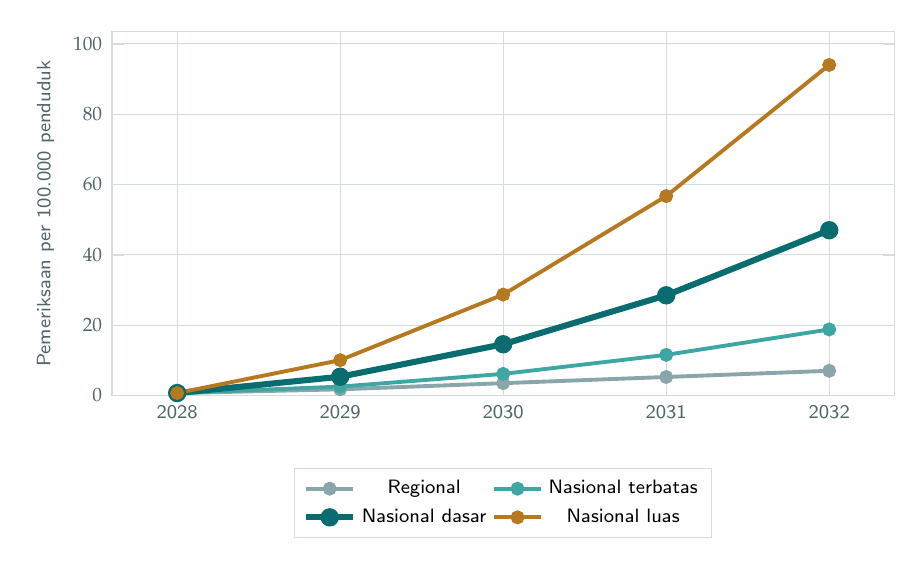
\begin{tikzpicture}
\begin{axis}[natplot,ymin=0,ylabel={Pemeriksaan per 100.000 penduduk},legend columns=2]
\addplot[color=sr1,line width=1.4pt,mark=*,mark size=1.8pt] coordinates {(1,0.70) (2,1.76) (3,3.51) (4,5.27) (5,7.03)};
\addplot[color=sr2,line width=1.4pt,mark=*,mark size=1.8pt] coordinates {(1,0.70) (2,2.53) (3,6.15) (4,11.56) (5,18.79)};
\addplot[color=sr3,line width=2.2pt,mark=*,mark size=2.2pt] coordinates {(1,0.70) (2,5.34) (3,14.58) (4,28.49) (5,47.00)};
\addplot[color=sr4,line width=1.4pt,mark=*,mark size=1.8pt] coordinates {(1,0.70) (2,10.05) (3,28.70) (4,56.70) (5,94.00)};
\legend{Regional,Nasional terbatas,Nasional dasar,Nasional luas}
\end{axis}
\end{tikzpicture}
\caption{Pemeriksaan per 100.000 penduduk menurut skenario.}
\label{fig:p100k}
\end{figure}

Angka pada skenario nasional dasar, yaitu Rp29,39 miliar (konservatif) sampai Rp191,52 miliar (panel kecil) selama lima tahun, atau Rp14,37 miliar sampai Rp93,66 miliar pada 2032, harus dibaca dengan empat batasan. Pertama, ia mengandaikan setiap kit menggantikan satu pemeriksaan pada harga pembanding, padahal sebagian pemeriksaan mungkin tidak akan terjadi tanpa kit yang lebih murah, sebagian lain menggantikan uji tusuk kulit yang harganya berbeda, dan cakupan kit lebih sempit. Kedua, selisih ini dinikmati pasien dan bukan nilai tambah yang tercatat dalam produk domestik bruto. Ketiga, penghematan hanya terjadi bila kit cukup akurat untuk dipakai klinisi, yang belum dibuktikan. Keempat, pembanding konservatif berasal dari satu rumah sakit dan pembanding panel kecil dari tiga fasilitas, sehingga keduanya tidak mewakili harga nasional. Kami tidak menyajikan perhitungan terhadap tarif Surabaya yang lebih tinggi, karena jenis tes dan jumlah alergennya tidak diketahui.

\subsection{Industri dan rantai pasok dalam negeri}

\begin{itemize}
\item \textbf{Produsen dan mitra.} Pada skenario nasional dasar, hasil operasi tahun ke-5 produsen adalah Rp11,74 miliar pada biaya tetap dasar, atau Rp9,04 miliar pada biaya tetap Rp3,0 miliar per tahun (sebelum pajak dan investasi awal; rincian pada studi kelayakan).
\item \textbf{Substitusi impor.} Pada 2019 sampai 2020, alat kesehatan impor menyumbang 88\% transaksi dan produk lokal sekitar 12\% (data Kementerian Kesehatan yang dilaporkan pada 2022) \cite{kemkes88}. Angka itu mencakup seluruh alat kesehatan, bukan diagnostik alergi, dan porsi impor khusus diagnostik alergi belum kami temukan. Nilai substitusi impor karena itu tidak dihitung.
\item \textbf{Kebijakan produk dalam negeri.} Pemerintah mendorong penggunaan alat kesehatan dalam negeri melalui program P3DN \cite{p3dn} dan e-katalog LKPP yang pada Oktober 2025 memuat 88.000 produk bersertifikat TKDN \cite{ekatalog}. Berlakunya kebijakan itu untuk produk dengan klasifikasi seperti kit ini belum dipastikan.
\item \textbf{Lapangan kerja, pajak, dan klaim JKN.} Tidak dihitung, karena rencana produksi, struktur mitra, dan skema penjaminan belum ditetapkan.
\end{itemize}

\section{Dampak sosial nasional}

\subsection{Akses dan pemerataan antarwilayah}

Kit dirancang agar dapat dipakai di layanan primer dan dibaca melalui aplikasi seluler, sehingga pemeriksaan awal tidak selalu menunggu rujukan ke spesialis. Bila validasi klinis mendukung, kit dapat membantu menyaring pasien yang perlu dirujuk. Klaim ini bersyarat: interpretasi hasil, penanganan reaksi, dan keputusan diagnosis tetap berada pada tenaga kesehatan, dan skor aplikasi tidak boleh dipakai sebagai diagnosis tunggal. Kekurangan spesialis di tingkat nasional \cite{kabarbursa} hanya menjadi konteks, bukan bukti bahwa kit mengisi kekurangan itu.

Jawa dan Sumatra memuat 77,78\% penduduk, sedangkan Maluku dan Papua hanya 3,17\% (Sensus Penduduk 2020 \cite{sensus}). Rencana peluncuran pada studi kelayakan bergerak dari Jawa ke wilayah lain karena alasan logistik dan kapasitas. Konsekuensinya, wilayah yang paling sulit mengakses spesialis dapat menjadi yang terakhir menerima kit. Dampak pemerataan karena itu tidak otomatis. Tabel~\ref{tab:reg} menunjukkan alokasi kit tahun ke-5 skenario nasional dasar bila sebanding dengan penduduk (asumsi), yang menjadi patokan indikator pemerataan pada Bagian 5.

\begin{table}[htbp]
\centering
\caption{Porsi penduduk menurut wilayah dan alokasi kit tahun ke-5 skenario nasional dasar (proporsional penduduk, asumsi).}
\label{tab:reg}
\tabstart
\begin{tabular}{@{}lrrr@{}}
\toprule
\hdrrow\tH{Wilayah} & \tH{Penduduk} & \tH{Kumulatif} & \tH{Kit tahun ke-5} \\
\midrule
Pulau Jawa & 56,10\% & 56,10\% & 75.062 \\
Sumatra & 21,68\% & 77,78\% & 29.008 \\
Sulawesi & 7,36\% & 85,14\% & 9.848 \\
Kalimantan & 6,15\% & 91,29\% & 8.229 \\
Bali dan Nusa Tenggara & 5,54\% & 96,83\% & 7.413 \\
Maluku dan Papua & 3,17\% & 100,00\% & 4.241 \\
\bottomrule
\end{tabular}
\end{table}

\subsection{Kenyamanan pada anak}

Pemeriksaan dengan patch tidak memerlukan penusukan kulit atau pengambilan darah, sehingga berpotensi lebih diterima oleh anak dan orang tua. Ini hipotesis berdasarkan cara kerja, dan belum diuji pada pasien. Pemakaian patch selama beberapa hari juga membawa beban tersendiri (kepatuhan memakai, iritasi kulit) yang perlu dicatat dalam uji.

\subsection{Kualitas hidup dan pantangan makanan}

Cay dkk. mengikuti 967 anak dengan alergi makanan yang didiagnosis alergolog di Amerika Serikat, dan menemukan bahwa beban psikososial anak dan pengasuh meningkat pada setiap tambahan alergi makanan \cite{cay}. Studi ini menunjukkan bahwa beban bertambah dengan jumlah alergi, bukan bahwa diagnosis melalui patch menguranginya. Hipotesis yang dapat diuji adalah bahwa diagnosis yang lebih tepat membantu keluarga membatasi pantangan pada makanan yang benar-benar bermasalah. Hipotesis itu bergantung pada akurasi diagnosis. Wai dkk. menegaskan bahwa diagnosis alergi makanan masih terus disempurnakan, termasuk penyempurnaan tes tusuk kulit dan IgE serum yang sudah ada \cite{wai}, sehingga kit baru perlu dibuktikan dengan pembanding yang sesuai.

\subsection{Risiko terhadap dampak}

\begin{itemize}
\item \textbf{Akurasi belum terbukti, dan kesalahan membesar pada skala nasional.} Hasil positif palsu dapat mendorong pantangan yang tidak perlu, dan negatif palsu dapat memberi rasa aman yang keliru. Pada skenario nasional dasar, setiap satu poin persen kesalahan klasifikasi pada tahun ke-5 berarti sekitar 1.338 pasien.
\item \textbf{Pembacaan foto.} Skor dari foto dapat dipengaruhi pencahayaan, kamera, dan warna kulit. Aplikasi perlu divalidasi pada ragam kondisi tersebut, terutama bila dipakai di banyak wilayah dengan perangkat berbeda.
\item \textbf{Data pribadi.} Foto kulit dan hasil pemeriksaan adalah data kesehatan. Pengelolaannya harus mengikuti Undang-Undang Nomor 27 Tahun 2022 tentang Pelindungan Data Pribadi.
\item \textbf{Keterjangkauan.} Harga kit rendah tidak menjamin tarif akhir rendah, karena margin ditentukan fasilitas. Pemantauan tarif akhir diperlukan (Tabel~\ref{tab:indikator}).
\item \textbf{Kesenjangan wilayah.} Peluncuran bertahap dari Jawa dapat menunda manfaat bagi wilayah timur (Bagian 4.1).
\end{itemize}

\section{Indikator dan rencana pengukuran}

Agar dampak dapat dibuktikan setelah izin edar, tim akan mengukur indikator pada Tabel~\ref{tab:indikator} pada tingkat fasilitas, wilayah, dan nasional. Semua indikator berstatus rencana, dan nilai awal (baseline) akan dikumpulkan pada fasilitas mitra sebelum kit dipakai.

\begin{table}[htbp]
\centering
\caption{Indikator dampak yang akan diukur.}
\label{tab:indikator}
\tabstart
\begin{tabular}{@{}L{3.0cm}L{4.4cm}L{3.9cm}L{3.2cm}@{}}
\toprule
\hdrrow\tH{Indikator} & \tH{Definisi} & \tH{Nilai awal dan sumber} & \tH{Frekuensi dan tingkat} \\
\midrule
Tarif akhir ke pasien & Harga pemeriksaan alergi yang ditagih fasilitas mitra, dengan dan tanpa kit & Daftar tarif fasilitas sebelum kit dipakai & Setiap semester; fasilitas dan provinsi \\
Akses pasien & Jumlah pasien yang diperiksa di layanan primer mitra, dan jarak atau waktu tunggu dibanding rujukan & Catatan registrasi fasilitas mitra & Setiap triwulan; fasilitas \\
Pemerataan wilayah & Porsi pemeriksaan per wilayah dibanding porsi penduduk (Tabel~\ref{tab:reg}) & Sensus Penduduk 2020 \cite{sensus}; data penjualan per wilayah & Setiap tahun; nasional \\
Ketepatan rujukan & Proporsi pasien yang dirujuk ke spesialis dan terkonfirmasi alergi & Catatan rujukan sebelum kit dipakai & Setiap semester; fasilitas \\
Akurasi diagnosis & Sensitivitas dan spesifisitas terhadap pembanding klinis yang ditetapkan protokol & Uji validasi klinis; belum ada & Pada tiap tahap uji; studi \\
Pantangan tidak perlu & Proporsi pasien yang menghentikan pantangan setelah konfirmasi klinis & Wawancara dan catatan klinik & Setiap semester; fasilitas \\
Konsistensi mutu & Variasi hasil antarbatch pada pengujian mutu & Sertifikat analisis tiap batch & Setiap batch; produksi \\
Kualitas hidup & Skor kuesioner kualitas hidup alergi makanan pada anak dan pengasuh & Pengukuran awal pada pasien mitra & Awal dan 6 bulan; pasien \\
\bottomrule
\end{tabular}
\end{table}

\section{Keterbatasan dokumen ini}

\begin{itemize}
\item Tidak ada data dampak yang berasal dari kit. Seluruh angka ekonomi adalah ilustrasi dari harga, tarif pembanding, dan skenario studi kelayakan.
\item Pembanding konservatif berasal dari satu paket rumah sakit (54 alergen, termasuk konsultasi) yang disetarakan secara pro rata, dan pembanding panel kecil dari tiga fasilitas. Tarif Surabaya dari agregator tidak merinci jenis tes dan jumlah alergen, dan harga Medicastore 2009 sudah tua.
\item Cakupan kit hanya sepuluh alergen. Perbandingan harga tidak menyamakan manfaat klinis dengan panel yang lebih luas.
\item Data luar negeri tidak dapat dikonversi ke Indonesia, dan dipakai hanya untuk menunjukkan arah.
\item Prevalensi asma Riskesdas 2018 dikutip melalui sumber sekunder. Prevalensi alergi susu sapi berasal dari kutipan media atas data IDAI.
\item Data impor 88\% berasal dari 2019 sampai 2020 dan mencakup seluruh alat kesehatan.
\item Hipotesis dampak sosial (akses, kenyamanan, pengurangan pantangan, pemerataan) belum diuji pada manusia.
\end{itemize}

\section{Data yang akan melengkapi dokumen ini}
\label{sec:data}

\begin{itemize}
\item Hasil validasi klinis (sensitivitas, spesifisitas, kejadian efek samping kulit).
\item Daftar harga resmi laboratorium dan fasilitas mitra di beberapa provinsi, lengkap dengan jenis tes, jumlah alergen, tanggal, dan cabang (panel kecil 10 sampai 20 alergen, uji tusuk kulit, dan IgE satuan).
\item Jumlah ahli alergi-imunologi dan fasilitas yang mampu melakukan uji alergi, menurut provinsi.
\item Proporsi diagnostik alergi yang diimpor, bila tersedia dari data kepabeanan atau asosiasi industri.
\item Klasifikasi regulasi produk, kepastian jalur izin edar, dan skema penjaminan JKN (lihat studi kelayakan skala nasional).
\end{itemize}

\begin{thebibliography}{99}\small\raggedright
\setlength{\itemsep}{2pt}
\bibitem{who} World Health Organization. Asthma, fact sheet, 28 April 2026. \url{https://www.who.int/news-room/fact-sheets/detail/asthma}
\bibitem{riskesdas} Kementerian Kesehatan RI. Riskesdas 2018 (asma terdiagnosis dokter, 2,4\%) dan Infodatin Penderita Asma di Indonesia, 2019. Dikutip melalui sumber sekunder.
\bibitem{antara} ANTARA. Prevalensi alergi susu sapi pada anak Indonesia 2 sampai 7,5\% (data Ikatan Dokter Anak Indonesia). 25 Juni 2024.
\bibitem{soegiarto} Soegiarto G, Abdullah MS, Damayanti LA, Suseno A, Effendi C. The prevalence of allergic diseases in school children of metropolitan city in Indonesia shows a similar pattern to that of developed countries. Asia Pac Allergy. 2019;9(2):e17. doi:10.5415/apallergy.2019.9.e17
\bibitem{norback} Norb\"ack D, Hashim JH, Hashim Z, et al. Fractional exhaled nitric oxide (FeNO) among school children in Java and Sumatra, Indonesia: associations with respiratory symptoms, house dust mite sensitization and the home environment. J Asthma. 2024;61(12):1772-1780. doi:10.1080/02770903.2024.2383627
\bibitem{kabarbursa} Kabarbursa.com. Menkes: RI masih butuh 29.000 dokter spesialis. 6 Mei 2024. \url{https://www.kabarbursa.com/market-hari-ini/menkes-ri-masih-butuh-29-000-dokter-spesialis}
\bibitem{jkn} Warta Ekonomi. Cakupan JKN tembus 98 persen penduduk Indonesia, BPJS catat peserta capai 282,7 juta jiwa. 27 Januari 2026. \url{https://wartaekonomi.co.id/read598290/cakupan-jkn-tembus-98-penduduk-indonesia-bpjs-catat-peserta-capai-2827-juta-jiwa}
\bibitem{bpjs} Bisnis.com. BPJS Kesehatan klaim kerja sama dengan 3.120 RS pada 2023. 14 Januari 2024. \url{https://finansial.bisnis.com/read/20240114/215/1732195/bpjs-kesehatan-klaim-kerja-sama-dengan-3120-rs-pada-2023}
\bibitem{sensus} Sekretariat Kabinet RI. Hasil Sensus Penduduk 2020; BPS: Meski lambat, ada pergeseran penduduk antarpulau. \url{https://setkab.go.id/hasil-sensus-penduduk-2020-bps-meski-lambat-ada-pergeseran-penduduk-antarpulau/}
\bibitem{alodokter} Alodokter. Tes Alergi, daftar tarif fasilitas di Surabaya. Diakses Oktober 2026. \url{https://www.alodokter.com/cari-rumah-sakit/kulit-dan-kelamin/tes-alergi/surabaya}
\bibitem{royal} Rumah Sakit Royal Progress. Paket Cek Alergi, IgE Atopy 54 Alergen (Rp2.200.000, termasuk konsultasi dokter). Diakses Oktober 2026. \url{https://oncare.royalprogress.com/en/s/rumah-sakit-royal-progress/detail-produk/paket-cek-alergi-ige-54-alergen}
\bibitem{medicastore} Medicastore. Tes Alergi (uji tusuk kulit 33 alergen Rp350.000 sampai Rp600.000; IgE spesifik Rp200.000 sampai Rp300.000 per alergen). 9 Januari 2009. \url{https://medicastore.com/artikel/1964/tes-alergi}
\bibitem{pramita} Laboratorium Klinik Pramita. Allergy Test Panels (IgE spesifik 96 alergen; harga tidak dicantumkan). 2 Oktober 2025. \url{https://pramita.co.id/en/inspiration/allergy-test-panels}
\bibitem{pramita2} Laboratorium Klinik Pramita. Food Allergy Check Panel (IgE spesifik 54 jenis; IgG Food Tolerance 46 jenis makanan; harga tidak dicantumkan). Diakses Oktober 2026. \url{https://pramita.co.id/en/inspiration/food-allergy-check-panel}
\bibitem{tim} Daftar harga tes alergi pada Siloam Hospitals, Tirta Medical Centre, RS Mitra Keluarga, Klinik Utama DR Indrajana, dan Laboratorium Klinik Pramita. Dihimpun Oktober 2026.
\bibitem{zuberbier} Zuberbier T, L\"otvall J, Simoens S, Subramanian SV, Church MK. Economic burden of inadequate management of allergic diseases in the European Union: a GA2LEN review. Allergy. 2014;69(10):1275-1279. doi:10.1111/all.12470. Dikutip dari siaran pers Wiley: \url{https://eurekalert.org/news-releases/494816}
\bibitem{gupta} Gupta R, Holdford D, Bilaver L, et al. The economic impact of childhood food allergy in the United States. JAMA Pediatr. 2013;167(11):1026-1031. doi:10.1001/jamapediatrics.2013.2376. Dikutip dari ringkasan: \url{https://www.newswise.com/articles/study-estimates-economic-impact-of-childhood-food-allergies}
\bibitem{cay} Cay M, Onal C, Herbert L, et al. Psychosocial burden of multiple IgE-mediated food allergies in pediatric patients and caregivers in the FORWARD study. Nutrients. 2026;18(11):1745. doi:10.3390/nu18111745
\bibitem{wai} Wai CYY, Santos AF, Leung TF, Sampson HA. Novel strategies for food allergy diagnosis. J Allergy Clin Immunol Pract. 2026;14(4):751-760. doi:10.1016/j.jaip.2025.11.022
\bibitem{kemkes88} Kementerian Kesehatan RI. Pemerintah targetkan 60 persen produksi alkes gunakan komponen lokal. 27 Agustus 2022. \url{https://www.kemkes.go.id/id/pemerintah-targetkan-60-persen-produksi-alkes-gunakan-komponen-lokal}
\bibitem{p3dn} BCA Sekuritas. Kemenperin perkuat pasar industri alat kesehatan lewat P3DN. 8 September 2025. \url{https://bcasekuritas.co.id/latest-news/news/kemenperin-perkuat-pasar-industri-alat-kesehatan-lewat-p3dn}
\bibitem{ekatalog} Kabarbursa.com. Pemerintah genjot produk lokal masuk e-katalog LKPP. 16 Oktober 2025. \url{https://www.kabarbursa.com/makro/pemerintah-genjot-produk-lokal-masuk-e-katalog-lkpp}
\end{thebibliography}

\end{document}
